\begin{frame}[fragile,label=ss-charm] 
\secframetitle{\ssCharm}
%--------------------------------------------------
\framesubtitle{MPI parallel programs: passing messages between processes}
%--------------------------------------------------
\begin{minipage}[t]{1.75in}
\begin{center}
\begin{minipage}{1.50in}
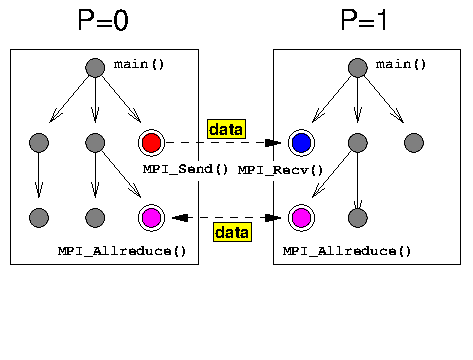
\includegraphics[width=1.50in]{mpi.pdf}\\
\vspace{-0.5in}
\centerline{\scriptsize\textbf{An MPI parallel program}}
\end{minipage}\\ \ \\
%\begin{minipage}{1.25in}
%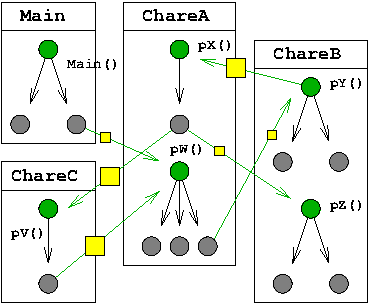
\includegraphics[width=1.25in]{charm.pdf}
%\ \\
%\centerline{\scriptsize\textbf{A Charm\pp\ parallel program}}
%\end{minipage}
\end{center}
\end{minipage} \ 
\begin{minipage}[t]{2.50in}
\vspace{-0.6in}
\begin{itemize}
\item MPI program
  \begin{itemize}
  \item decomposed by \blueit{processes}
  \item calls MPI library
  \item communicate / synchronize
  \end{itemize}
\ \\ \pause
\item MPI runtime system
  \begin{itemize}
  \item sends data between processes
  \item synchronizes between processes
  \end{itemize} \pause
\item Additional features
\begin{itemize}
\item MPI-2: Parallel I/O, remote DMA,
one-sided communication
\item MPI-3: fault-tolerance, hybrid programming, persistence
\end{itemize}
\end{itemize}
\end{minipage}
\end{frame}
